%
% CHAPTER: Preliminaries
%

\chapterimage{Koenigsberg_Map_by_Bering_1613.pdf} % Chapter heading image

\chapter{Discrete Mathematics}
\label{chap:Discrete_Mathematics}

\begin{quote}
\begin{flushright}
\emph{Mathematics may be defined as the subject in which\\
we never know what we are talking about,\\
nor whether what we are saying is true.}\\
Bertrand Russell
\end{flushright}
\end{quote}
\bigskip

The majority of mathematical concepts used throughout this book belong to the domain of \emph{discrete mathematics}. This field focuses on mathematical objects that take on distinct, separate values, as opposed to continuous ones. In this book, we make use of various discrete structures, including integers, strings, graphs, and computer programs. A key feature of discrete sets is their countability, meaning they can be put into one-to-one correspondence with the natural numbers. By contrast, continuous mathematics, such as calculus, will play only a minimal role in the theoretical development of the theory of nescience.

Our primary interest in discrete mathematics arises from its direct relevance to computation. The theory of nescience draws upon various aspects of computer science, including algorithms, coding, and string complexity. Computers operate in discrete steps and manipulate information stored in discrete memory units. Our interest in computers stems from the aspiration to apply our theoretical framework to a broad range of real-world entities. We consider computers to be the most suitable tools for modeling the world around us. While pure mathematics often engages with abstract objects independent of their representations, the theory of nescience places significant emphasis on the representation (or encoding) of objects.

This chapter provides a brief overview of the fundamental concepts of discrete mathematics, introducing topics such as sets, strings and languages, counting methods, matrices, and graphs. While we do not present formal definitions or prove theorems in this overview, these subjects lay the groundwork for the theories and ideas explored in later sections. Discrete mathematics is a broad and diverse field; here, we focus only on those elements essential for understanding the theory of nescience. More advanced topics (such as computability, information theory, and complexity) require a deeper treatment and are addressed in dedicated chapters.

The References section provides a list of recommended books that explore the topics introduced in this chapter in greater depth. Readers interested in further developing their understanding can use this list to delve more deeply into each subject, thereby complementing the foundational overview presented here.

%
% Section: Sets
%

\section{Sets, Relations and Functions}
\label{sec:sets}

The sets of \emph{natural}\index{Set of natural numbers}, \emph{integer}\index{Set of integers}, \emph{rational}\index{Set of rationals}, and \emph{real}\index{Set of real numbers} numbers are denoted by $\mathbb{N}$, $\mathbb{Z}$, $\mathbb{Q}$, and $\mathbb{R}$, respectively. Each of these sets includes the number $0$. The \emph{positive integers}\index{Set of positive integers} are represented by $\mathbb{Z}^+$, and the \emph{positive reals}\index{Set of positive reals} by $\mathbb{R}^+$; both sets also include $0$. Let $A$ be a \emph{set}\index{Set}. We indicate that $x$ is an \emph{element}\index{Element of a set} of $A$ using the notation $x \in A$, and that $x$ is not an element of $A$ with $x \notin A$. Elements of a set can be listed explicitly using braces, as in $A = \{0, 1, 2, 3\}$, or defined by a condition using \emph{set-builder}\index{Set formation notation} notation, for example, $A = \{x \in \mathbb{N} : x < 4\}$, provided that the \emph{universe}\index{Universe of a set} of discourse is clearly specified.

Suppose $A$ and $B$ are two sets. We use the notation $A = B$ to indicate that the sets are \emph{equal}\index{Equal sets}. The expression $A \subseteq B$ signifies that $A$ is a \emph{subset or equal}\index{Subset} to $B$, while $A \subset B$ denotes that $A$ is a \emph{proper subset}\index{Proper subset} of $B$ (meaning that $A$ is contained in $B$ but is not equal to $B$). The condition $A = B$ holds if and only if both $A \subseteq B$ and $B \subseteq A$ are true. The symbol $\varnothing$ denotes the \emph{empty set}\index{Empty set}, which is the set containing no elements.

\begin{example}
For every set $A$, we have that $\varnothing \subseteq A$ and $A \subseteq A$.
\end{example}

The term \emph{cardinality}\index{Cardinality of a set} refers to the number of elements in a finite set $A$, denoted by $d(A)$. Accordingly, the cardinality of the empty set $\varnothing$ is 0, since it contains no elements. For any two sets $A$ and $B$, the notation $A \cup B$ denotes the \emph{union}\index{Union of sets} of $A$ and $B$, while $A \cap B$ represents their \emph{intersection}\index{Intersection of sets}. For a collection of $n$ sets $A_1, A_2, \ldots, A_n$, we write their union and intersection as $\cup_{i=1}^n A_i$ and $\cap_{i=1}^n A_i$, respectively. For an arbitrary collection of sets indexed by a set $I$, we use the notations $\cup_{i \in I} A_i$ and $\cap_{i \in I} A_i$. When dealing with an infinite collection of sets, we may use the shorthand $\cup_{i=1}^{\infty} A_i$ and $\cap_{i=1}^{\infty} A_i$. Occasionally, we will make use of \emph{Venn diagrams}\index{Venn diagram} to visually represent set operations, as illustrated in Figure \ref{fig:Venn-diagram}.

\begin{figure}[t]
\centering
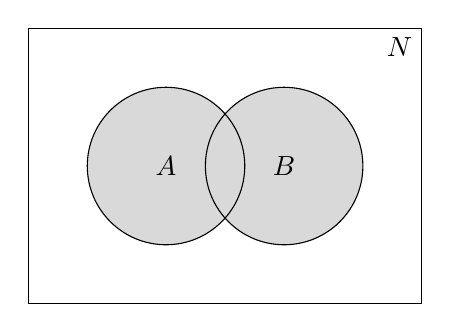
\begin{tikzpicture}

    % Rectangle with label
    \draw (0,0) rectangle (5,3.5) node[below left] {$\mathbb{N}$};
    
    \fill[gray!30] (1.75,1.75) circle (1);
    \fill[gray!30] (3.25,1.75) circle (1);

    \node[draw, circle, minimum width=2cm, label=center:{$A$}] at (1.75, 1.75) {};
    \node[draw, circle, minimum width=2cm, label=center:{$B$}] at (3.25, 1.75) {};

\end{tikzpicture}
\caption{\label{fig:Venn-diagram}Representation of $A \cup B$ as a Venn Diagram}
\end{figure}

Given any two sets $A$ and $B$, the \emph{set difference}\index{Set difference} is denoted by $A \backslash B$, and the \emph{complement}\index{Complement of a set} of the set $A$ is written as $A^c$. \emph{De Morgan's laws}\index{De Morgan's laws} state that for any sets $A$ and $B$, we have $\left( A \cup B \right)^c = A^c \cap B^c$ and $\left( A \cap B \right)^c = A^c \cup B^c$.

Two sets $A$ and $B$ are said to be \emph{disjoint}\index{Disjoint sets} if their intersection is empty, i.e., $A \cap B = \varnothing$. A collection of sets $A_1, A_2, \ldots, A_n$ is disjoint if $A_i \cap A_j = \varnothing$ for all $i \neq j$. A \emph{partition}\index{Partition of a set} of a set $A$ is a collection of nonempty, pairwise disjoint subsets $A_1, A_2, \ldots, A_n$ such that $A = \cup_{i=1}^n A_i$. The \emph{power set}\index{Power set} of $A$, denoted by $\mathcal{P}(A)$, is the set of all possible subsets of $A$. If the cardinality of $A$ is $n$, i.e., $d(A) = n$, then the cardinality of its power set is $2^n$, so $d\left( \mathcal{P}(A) \right) = 2^n$.

\begin{example}
Given the set $A = \{1, 2, 3\}$, its power set is:
\[
\mathcal{P}(A) = \{\varnothing, \{1\}, \{2\}, \{3\}, \{1,2\}, \{1,3\}, \{2,3\}, A\}
\]
\end{example}

Consider a non-empty set $A$ and a collection $\mathcal{F}$ of subsets of $A$. The pair $\left( A, \mathcal{F} \right)$ is called a \emph{field}\index{Field of sets} over $A$ if it satisfies the following conditions: it contains the empty set, that is, $\varnothing \in \mathcal{F}$; it is closed under complementation, meaning that for every $F \in \mathcal{F}$, the complement $F^c$ also belongs to $\mathcal{F}$; and it is closed under finite unions, meaning that for any subsets $F_1, \ldots, F_n \in \mathcal{F}$, the union $F_1 \cup \ldots \cup F_n$ is also in $\mathcal{F}$. Additionally, it can be shown that a field also satisfies two further properties: the universal set $A$ itself belongs to $\mathcal{F}$, and it is closed under finite intersections, so that $F_1 \cap \ldots \cap F_n \in \mathcal{F}$ for all subsets $F_1, \ldots, F_n \in \mathcal{F}$.

% Relations

Consider two elements, $x$ and $y$. An \emph{ordered pair}\index{Ordered pair}, denoted as $(x, y)$, is a pairing in which the order of the elements matters. Generalizing this idea, an \emph{n-tuple}\index{n-tuple} is an ordered sequence of $n$ elements, written as $(x_1, \ldots, x_n)$. The \emph{Cartesian product}\index{Cartesian product} of two sets $A$ and $B$, denoted by $A \times B$, is the set of all ordered pairs $(x, y)$ such that $x \in A$ and $y \in B$. This concept extends naturally to $n$ sets $A_1, A_2, \dots, A_n$, where the Cartesian product is expressed as $A_1 \times A_2 \times \dots \times A_n$. Additionally, the \emph{n-fold Cartesian product} of a set $A$ with itself is denoted as $A^n$.

Let $R$ be a subset of the Cartesian product of a set $A$ with itself, i.e., $R \subseteq A \times A$. Such a subset is called a \emph{binary relation}\index{Binary relation}. We write $aRb$ to indicate that the ordered pair $(a, b)$ belongs to $R$. A binary relation is said to be \emph{reflexive}\index{Reflexive relation} if, for every element $a \in A$, it holds that $aRa$. It is called \emph{symmetric}\index{Symmetric relation} if, for all $a, b \in A$, the condition $aRb$ implies $bRa$. A relation is \emph{antisymmetric}\index{Antisymmetric relation} if, for all $a, b \in A$, the coexistence of $aRb$ and $bRa$ implies $a = b$. It is \emph{transitive}\index{Transitive relation} if, for all $a, b, c \in A$, the conditions $aRb$ and $bRc$ together imply $aRc$. A relation is \emph{total}\index{Total relation} if, for every pair $a, b \in A$, either $aRb$ or $bRa$ holds. Binary relations can also be defined between two different sets $A$ and $B$, in which case $R$ is a subset of $A \times B$. Furthermore, the concept can be generalized to \emph{n-ary} relations, represented as $R \subseteq A_1 \times A_2 \times \dots \times A_n$.

Let $R$ be a binary relation that is a subset of the Cartesian product $A \times A$, i.e., $R \subseteq A \times A$. If this relation is reflexive, symmetric, and transitive, it is called an \emph{equivalence relation}\index{Equivalence relation}, typically denoted by the symbol $\sim$. Under an equivalence relation, two elements $a, b \in A$ are said to be \emph{equivalent}\index{Equivalent elements} if $a \sim b$. The \emph{equivalence class}\index{Equivalence class} of an element $a$, denoted by $[a]$, is the set of all elements in $A$ that are equivalent to $a$. That is, the equivalence class of $a$ is defined as $[a] := \{ b \in A : a \sim b \}$. An equivalence relation partitions the set $A$ into disjoint subsets known as \emph{equivalence classes}, collectively forming what is called the \emph{quotient set}\index{Quotient set}. The quotient set is denoted by $A / {\mathord {\sim }}$ and is defined as the set of all equivalence classes: $A / {\mathord {\sim }} := { [a] : a \in A }$.

A binary relation that is reflexive, transitive, and antisymmetric is known as a \emph{partial order}\index{Partial order}, typically denoted by the symbol $\preceq$. A set equipped with a partial order is called a \emph{partially ordered set}\index{Partially ordered set}, or \emph{poset}\index{poset} for short. In a poset, an element $a \in A$ is considered \emph{minimal}\index{Minimal element} if there is no element $b \in A$ such that $b \preceq a$ and $b \neq a$. Similarly, an element $a$ is said to be \emph{maximal}\index{Maximal element} if there is no element $b \in A$ such that $a \preceq b$ and $b \neq a$. A relation that is reflexive, transitive, antisymmetric, and total is called a \emph{total order}\index{Total order}, often denoted by the symbol $\leq$. A set endowed with a total order is referred to as a \emph{totally ordered set}\index{Totally ordered set}. In such a set $A$, the \emph{maximum element}\index{Maximum element}, denoted by $\max(A)$, satisfies $\max(A) \geq x$ for all $x \in A$, and the \emph{minimum element}\index{Minimum element}, denoted by $\min(A)$, satisfies $\min(A) \leq x$ for all $x \in A$.

\begin{example}
Let $R$ be a relation that is a subset of the Cartesian product of the set of natural numbers $\mathbb{N}$ with itself, i.e., $R \subset \mathbb{N} \times \mathbb{N}$. In this relation, an ordered pair $(a, b)$ belongs to $R$ if and only if $a$ is a divisor of $b$. The set $\mathbb{N}$, together with the relation $R$, forms a partially ordered set. In this context, 1 is the unique minimal element, and every prime (e.g. 11) is maximal.
\end{example}

% Functions

A \emph{function}\index{Function} is defined as a binary relation $f \subseteq A \times B$ such that for each element $x \in A$, there exists at most one $y \in B$ for which $\left(x, y\right) \in f$. In this context, elements $\left(x, y\right) \in f$ are written as $f(x) = y$, and the function is denoted by $f : A \rightarrow B$. The set $A$ is called the \emph{domain}\index{Domain} of $f$, and $B$ is the \emph{codomain}\index{Codomain}. The set ${ y \in B : \exists x \in A \text{ such that } f(x) = y }$ is known as the \emph{range}\index{Range} of $f$. If the relation is not defined for every $x \in A$, the function is called a \emph{partial function}\index{Partial function}, and we write $f(x) \uparrow$ to indicate that $f$ is undefined at $x$.

A function is said to be \emph{injective}\index{Injective function} if, for all elements $x$ and $y$, the condition $f(x) = f(y)$ implies that $x = y$. A function is \emph{surjective}\index{Surjective function} if, for every $y$ in the codomain, there exists at least one $x$ in the domain such that $f(x) = y$. A function is described as \emph{bijective}\index{Bijective function} if it is both injective and surjective. The \emph{identity}\index{Identity function} function $I_A : A \rightarrow A$, defined by $I_A(a) = a$ for all $a \in A$, is an example of a bijective function. These concepts (function, partial function, injective, surjective, and bijective) can be extended to $n$-ary functions, which are functions of the form $f: A_1 \times A_2 \times \dots \times A_n \rightarrow B$.

The \emph{inverse}\index{Inverse function} of a bijective function $f$, denoted by $f^{-1}$, is defined as $f(f^{-1}(x)) = f^{-1}(f(x)) = x$, for all $x$ in the domain of $f^{-1}$ and the range of $f$, respectively. Given two functions $f$ and $g$, where the domain of $f$ includes the range of $g$, the \emph{composition}\index{Composition} of $f$ with $g$, denoted by $f \circ g$, is defined as $(f \circ g)(x) = f(g(x))$.

\begin{example}
In Section \ref{sec:computable_functions}, we will explore an alternative interpretation of a function as a procedure or algorithm that assigns an element of $B$ to each element of $A$. For example, the following C code defines a partial function from $\mathbb{R}$ to $\mathbb{R}$, which is partial because $inv(0) \uparrow$:
\begin{verbatim}
    double inv(double x) {
        return 1 / x;
    }
\end{verbatim}
\end{example}

The \emph{characteristic function}\index{Characteristic function} of a set $A$ is denoted by $1_A : A \rightarrow \{1, 0\}$, where $1_A(x) = 1$ if $x \in A$ and $1_A(x) = 0$ otherwise.

An infinite set $A$ is said to be \emph{countable}\index{Countable set} if there exists a bijective function that maps the elements of $A$ onto the set of natural numbers $\mathbb{N}$. In contrast, a set is considered \emph{uncountable}\index{Uncountable set} if it is neither finite nor countable. A set is said to have \emph{countably many}\index{Countably many set} elements if it is either finite or countably infinite.

\begin{example}
The sets $\mathbb{N}$, $\mathbb{Z}$, and $\mathbb{Q}$ are countable, whereas $\mathbb{R}$ is uncountable.
\end{example}

Considering a real number $x \in \mathbb{R}$, its \emph{absolute value}\index{Absolute value}, denoted by $\mid x \mid$, is defined as $x$ if $x \geq 0$ and $-x$ if $x < 0$. The \emph{ceiling}\index{Ceil} function of $x$, written as $\lceil x \rceil$, is the smallest integer greater than or equal to $x$. The \emph{floor}\index{Floor} function of $x$, denoted by $\lfloor x \rfloor$, is the largest integer less than or equal to $x$. Given two positive integers $a$ and $b$, the \emph{modulo}\index{Modulo} operation, written as $a \bmod b$, yields the remainder when $a$ is divided by $b$.

For two functions $f$ and $g$ defined as $f, g : \mathbb{N} \rightarrow \mathbb{R}^{+}$, we say that $f(n)$ is of the \emph{order of}\index{Order of a function} $g(n)$, denoted $f(n) = O(g(n))$, if there exist positive constants $c > 0$ and $m$ such that $f(n) \leq c g(n)$ for all integers $n \geq m$. In this context, $g$ is called an \emph{upper bound}\index{Upper bound of a function} for $f$.

%
% Section: Strings and Languages
%

\section{Strings and Languages}
\label{sec:strings}

Consider a non-empty finite set $\mathcal{S} = \{ s_1, s_2, \ldots, s_q \}$, referred to as the \emph{alphabet}\index{Alphabet}. The elements of this set are called \emph{symbols}\index{Symbols}. A \emph{sequence}\index{Sequence of symbols} over $\mathcal{S}$ is defined as an ordered arrangement of symbols $x_1 x_2 \dots x_n$, where each $x_i$ belongs to $\mathcal{S}$. In the special case where the alphabet is $\mathcal{B} = \{0, 1\}$, such sequences are known as \emph{binary sequences}\index{Binary sequence}. We use the term \emph{string}\index{String} to denote a finite sequence. This book primarily focuses on binary strings.

The \emph{length}\index{Length of a string} of a string $s$, denoted by $l(s)$, refers to the total number of symbols contained in $s$. The symbol $\lambda$ is used to denote the \emph{empty string}\index{Empty string}, which is defined as the unique string over $\mathcal{S}$ with length 0. Given a symbol $x \in \mathcal{S}$, the string consisting of $x$ repeated $n$ times is denoted by $x^n$. If $s = x_1 x_2 \dots x_n$ is a string, its \emph{reverse}\index{Reverse string}, denoted by $s^R$, is given by $x_n x_{n-1} \dots x_1$.

The set of all strings $s\_{1}s\_{2}\ldots s\_{n}$ of length $n$ over the alphabet $\mathcal{S}$ is denoted by $\mathcal{S}^{n}$\footnote{It is important to avoid confusing the set of strings of length $n$ over an alphabet, $\mathcal{S}^n$, with the $n$-fold Cartesian product of a set, $S^n$. The use of calligraphic fonts helps distinguish between alphabets and other sets.}. We denote by $\mathcal{S}^{+}$ the union of all $\mathcal{S}^{n}$ for $n \geq 1$, and by $\mathcal{S}^{\ast}$ the set $\mathcal{S}^{+} \cup {\lambda}$. Note that all strings in $\mathcal{S}^{\ast}$ have finite length. The term \emph{Kleene closure}\index{Kleene closure} refers to $\mathcal{S}^{\ast}$.

\begin{example}
The following relations hold: the cardinality of the set of binary strings of length $n$ is $d \left( \left\{ s \in \mathcal{B}^{\ast} : l(s) = n \right\} \right) = 2^n$, and the cardinality of the set of binary strings of length up to $n$ is $d \left( \left\{ s \in \mathcal{B}^{\ast} : l(s) \leq n \right\} \right) = 2^{n+1}-1$.
\end{example}

Given two strings $s$ and $t$ from $\mathcal{S}^{\ast}$, the \emph{concatenation}\index{String concatenation} of $s$ and $t$, denoted as $st$, is the sequence obtained by placing the sequence of symbols in $t$ immediately after the sequence in $s$. Consequently, the length of the concatenated string, $l(st)$, is the sum of the lengths of $s$ and $t$. This indicates that $\mathcal{S}^\ast$ is closed under the operation of concatenation. Moreover, the set $\mathcal{S}^\ast$, together with concatenation, forms a \emph{free monoid}\index{Free monoid}. This means that concatenation is associative ($s(tr) = (st)r$), and that there exists an identity element, specifically, the empty string $\lambda$, for which $\lambda a = a \lambda = a$ holds for any string $a$.

A string $s$ is called a \emph{substring}\index{Substring} of a string $t$ if there exist strings $u$ and $v$ (possibly empty) such that $t = usv$. If there exists a string $u$ such that $t = su$, then $s$ is said to be a \emph{prefix}\index{Prefix string} of $t$, denoted by $s <_p t$. A subset $S \subset \mathcal{S}^{\ast}$ is described as \emph{prefix-free}\index{Prefix free set} if, for any $s, t \in S$, the condition $s <_p t$ implies $s = t$. Given two sets of strings $S, T \subset \mathcal{S}^{\ast}$, the (left) \emph{quotient}\index{String quotient} $S^{-1}T$ is defined as the set of residual strings obtained from $T$ by removing a prefix in $S$; formally, $S^{-1}T = \{\, t \mid st \in T \land s \in S \,\}$.

We denote the \emph{self-delimited}\index{Self delimited string} form of a string $s \in \mathcal{S}^{\ast}$ by $\bar{s}$, and define it as $\bar{s} = 1^{l(s)}0s$. Consequently, the length of $\bar{s}$, denoted $l(\bar{s})$, is given by $l(\bar{s}) = 2l(s) + 1$, meaning it is twice the length of $s$ plus one.

\begin{example}
The set $\bar{\mathcal{S}^{\ast}}$, consisting of all self-delimited strings from $\mathcal{S}^{\ast}$, is prefix-free.
\end{example}

In cases where $\mathcal{S}$ is a totally ordered set, we can define a total order on $\mathcal{S}^{\ast}$. This ordering, known as \emph{shortlex ordering}\index{Shortlex ordering}, arranges sequences primarily by length, with shorter sequences appearing first. Among sequences of the same length, lexicographical order is used to break ties.

\begin{example}
Given $\mathcal{S} = {a, b, c}$ with $a < b < c$, the shortlex order on $\mathcal{S}^{\ast}$ produces the sequence $\lambda < a < b < c < aa < ab < \ldots < cc < aaa < aab < \ldots < ccc < \ldots$
\end{example}

For any arbitrary object $O$, we use the notation $\left\langle O \right\rangle$ to denote its string based representation, assuming the existence of a standard encoding scheme. For objects $O_{1}, O_{2}, \ldots, O_{k}$, the expression $\left\langle O_1 O_2 \ldots O_k \right\rangle$ refers to the plain concatenation of their string representations: $\left\langle O_1 \right\rangle \left\langle O_2 \right\rangle \ldots \left\langle O_k \right\rangle$. By contrast, the notation $\left\langle O_1, O_2, \ldots, O_k \right\rangle$ indicates a structured concatenation that allows for the decoding and unique identification of each individual object. For example, this may be implemented as $\bar{\left\langle O_1 \right\rangle} \bar{\left\langle O_2 \right\rangle} \ldots \bar{\left\langle O_k \right\rangle}$.

\begin{example}
Natural numbers can be represented by binary strings via the following encoding method: $\langle 0 \rangle = \lambda$, $\langle 1 \rangle \rightarrow 0$, $\langle 2 \rangle \rightarrow 1$, $\langle 3 \rangle \rightarrow 00$, $\langle 4 \rangle \rightarrow 01$, $\langle 5 \rangle \rightarrow 10$, $\langle 6 \rangle \rightarrow 11$, $7 \rightarrow 000$, and so on. Therefore, the pair of numbers $\left\langle 3, 7 \right\rangle$ would be represented as $110001110000$. Given this particular encoding, it follows that $l \left( \langle n \rangle \right) = \lfloor \log_2 (n + 1) \rfloor$.
\end{example}

A \emph{language}\index{Language}, denoted by $L$, over an alphabet $\mathcal{S}$, is defined as a subset of strings, that is, $L \subseteq \mathcal{S}^{\ast}$. The individual elements of $L$ are called \emph{words}\index{Words of a language}. The unique language that contains no words is referred to as the \emph{empty language}\index{Empty language}, and is denoted by $L = \varnothing$.

Consider two languages $L_1$ and $L_2$ over a common alphabet $\mathcal{S}$. Several standard operations can be applied to these languages. The \emph{union} of $L_1$ and $L_2$ is defined as $L_1 \cup L_2 = { w \in \mathcal{S}^{\ast} \mid w \in L_1 \text{ or } w \in L_2 }$. The \emph{intersection} of $L_1$ and $L_2$ is given by $L_1 \cap L_2 = { w \in \mathcal{S}^{\ast} \mid w \in L_1 \text{ and } w \in L_2 }$. The \emph{complement} of $L_1$ is defined as $\overline{L_1} = { w \in \mathcal{S}^{\ast} \mid w \notin L_1 }$. Finally, the \emph{Kleene closure} of $L_1$, denoted $L_1^\ast$, is defined as $L_1^\ast = { \lambda } \cup { wz \mid w \in L_1 \text{ and } z \in L_1^\ast }$.

Languages can be systematically generated using a finite set of string rewriting rules, commonly referred to as grammars. A \emph{grammar}\index{Grammar}, denoted by $G$, is defined as a 4-tuple $(N, \Sigma, P, S)$, where: $N \subseteq \mathcal{S}$ is a finite set of \emph{nonterminal symbols}\index{Non-terminal symbol}; $\Sigma \subseteq \mathcal{S}$ is a finite set of \emph{terminal symbols}\index{Terminal symbol}; $P$ is a finite set of \emph{production rules}\index{Production rule} of the form $(\Sigma \cup N)^\ast N (\Sigma \cup N)^\ast \rightarrow (\Sigma \cup N)^\ast$; and $S \in N$ is a distinguished \emph{start symbol}\index{Start symbol}. Each production rule allows one string of symbols to be rewritten into another, beginning with the start symbol and proceeding through successive applications of the rules.

\begin{example}
\label{ex:context_free_grammar}
Consider the alphabet $\mathcal{S} = \{ S, a, b \}$, and define the grammar $(N, \Sigma, P, S)$ where $N = \{ S \}$, $\Sigma = \{ a, b \}$, $P = \{ S \rightarrow aSb, S \rightarrow ba \}$, and the start symbol is $S \in N$. This grammar generates the language $L = \{ a^nbab^n \mid n\geq0 \} = \{ ba, abab, aababb, aaababbb, \ldots \}$.
\end{example}

The \emph{Chomsky hierarchy}\index{Chomsky hierarchy} is a classification scheme for grammars, organized according to their expressive power, that is, the types of languages they are capable of generating. The hierarchy, arranged from the most to the least restrictive class of grammars, is described as follows (where $a$ denotes a terminal symbol; $A, B$ are nonterminal symbols; and $\alpha, \beta$, and $\gamma$ are strings composed of terminals and/or nonterminals):

\begin{description}
\item[Type-3] Known as \emph{regular grammars}\index{Regular grammar}. In these grammars, the left-hand side of each production rule consists of a single nonterminal symbol. The right-hand side must be either the empty string, a single terminal symbol, or a terminal symbol followed by a nonterminal symbol. Formally, the rules are of the form $A \rightarrow \lambda$, $A \rightarrow a$, or $A \rightarrow aB$.

\item[Type-2] Referred to as \emph{context-free grammars}\index{Context-free grammar}. In this class, the left-hand side of each production rule is exactly one nonterminal symbol. The general form of the rules is $A \rightarrow \alpha$.

\item[Type-1] These are \emph{context-sensitive grammars}\index{Context sensitive grammar}. Here, production rules allow a nonterminal to be replaced by a string in a specific context. The rules take the form $\alpha A \beta \rightarrow \alpha \gamma \beta$.

\item[Type-0] This category includes \emph{recursively enumerable grammars}\index{Recursively enumerable grammar}, which place no restrictions on the structure of production rules. These can be written in the general form $\gamma \rightarrow \alpha$.
\end{description}

\begin{example}
The grammar presented in Example \ref{ex:context_free_grammar} is a Type-2 grammar, that is, a context-free grammar.
\end{example}

The \emph{Backus-Naur form}\index{Backus-Naur form} (BNF) is a notation system specifically designed to describe context-free grammars. It is widely used in computer science to formally specify the syntax of programming languages and communication protocols. A BNF grammar consists of a set of production rules structured as follows:

\begin{verbatim}
    <symbol> ::= __expression__
\end{verbatim}

Here, \texttt{<symbol>} denotes a non-terminal symbol, \texttt{\_\_expression\_\_} represents a sequence of terminal and/or non-terminal symbols, and \texttt{::=} signifies that the symbol on the left-hand side can be replaced by the expression on the right. Multiple alternatives for the expression can be provided in a single rule by separating them with a vertical bar \texttt{|}, indicating that any one of the alternatives may be chosen during substitution. Symbols that never appear on the left-hand side of any production rule are considered terminal symbols. In contrast, those that do appear on the left-hand side are non-terminal symbols and are conventionally enclosed in angle brackets \texttt{<>}. The non-terminal symbol on the left-hand side of the first production rule is designated as the start symbol.

\begin{example}
The grammar introduced in Example \ref{ex:context_free_grammar} can be expressed in Backus-Naur form using the following production rule:
\begin{verbatim}
    <string> ::= a <string> b | ba
\end{verbatim}
\end{example}

%
% Section: Counting Methods
%

\section{Counting Methods}
\label{sec:counting}

\emph{Combinatorics}\index{Combinatorics}, a specialized branch of mathematics, is primarily concerned with the study of discrete objects and the relationships among them. Its central themes include the counting, arrangement, and selection of such objects, along with the methods used to carry out these tasks. Combinatorics provides a powerful set of tools for analyzing large collections of objects that satisfy specific properties. In this section, we revisit the most important results in combinatorics, focusing on their interpretation in terms of sets and ordered lists.

The \emph{multiplication rule}\index{Multiplication rule} is a fundamental principle that determines the number of possible outcomes in the Cartesian product of sets. According to this rule, if there are $k$ sets $A_1, A_2, \ldots, A_k$, and each set $A_i$ contains $n_i$ elements (for $i = 1, \ldots, k$), then the Cartesian product $A_1 \times A_2 \times \ldots \times A_k$ contains exactly $n_1 n_2 \ldots n_k$ elements. In particular, if a set $A$ has $n$ elements, then the $k$-fold Cartesian product $A^k$ contains $n^k$ elements.

The \emph{inclusion-exclusion principle}\index{Inclusion-exclusion principle} determines the cardinality of the union of multiple sets based on the sizes of the individual sets and all possible intersections among them. Given $k$ sets $A_1, A_2, \ldots, A_k$, the formula is:
\begin{equation*}
\begin{split}
d \left( \bigcup_{i=1}^k A_i \right) & = \sum_{i=1}^k d \left( A_i \right) - \sum_{i<j} d \left( A_i \cap A_j \right) + \sum_{i<j<l} d \left( A_i \cap A_j \cap A_l \right) - \\
& - \sum_{i<j<l<m} d \left( A_i \cap A_j \cap A_l \cap A_m \right) + \ldots +  (-1)^{k+1} d \left( A_1 \cap \ldots \cap A_k \right) 
\end{split}
\end{equation*}
\emph{Permutations}\index{Permutations} refer to the number of distinct ways in which the elements of a set can be arranged. Let $A$ be a set with $n$ elements. The number of ordered selections of $k$ elements from $n$ distinct elements without replacement, denoted by $P_{n,k}$, is given by $P_{n,k} = n \left( n-1 \right) \ldots \left( n-k+1 \right)$. In the case where $k = n$, the total number of permutations is $P_{n,n} = n \left( n-1 \right) \cdots 1 = n!$ where $n!$ is read as "$n$ factorial".

\begin{example}
Consider the set $\{a, b, c\}$. There are six distinct permutations of its elements: $\{a, b, c\}$, $\{a, c, b\}$, $\{b, a, c\}$, $\{b, c, a\}$, $\{c, a, b\}$, and $\{c, b, a\}$. Each permutation represents a unique ordering of the elements in the original set. 
\end{example}

The \emph{pigeonhole principle}\index{Pigeonhole principle} is a simple yet powerful concept. It asserts that if there are more pigeons than pigeonholes, then at least one pigeonhole must contain more than one pigeon. More formally, if $n$ items are distributed among $m$ containers and $n > m$, then at least one container must hold more than one item.

The logarithmic form of \emph{Stirling's}\index{Stirling's formula} approximation is particularly effective for estimating large factorials:
\[
\log\left(n!\right) \approx \frac{1}{2}\log\left(2\pi\right)+\left(n+\frac{1}{2}\right)\log\left(n\right)-n
\]

Numerous counting problems involve determining the number of subsets of a specific size within a given set. For a set with $n$ elements, the total number of possible subsets is $2^n$, including both the empty set and the set itself. The number of subsets of size $k$, also known as the number of \emph{combinations}\index{Combinations} of $k$ elements from a set of $n$, is denoted by $C_{n,k}$ and computed using the formula $C_{n,k} = \frac{P_{n,k}}{k!} = \frac{n!}{k!(n-k)!}
$. The symbol ${n \choose k}$ also represents the value $C_{n,k}$, which is known as the \emph{binomial coefficient}\index{Binomial coefficient}. It is known that ${n \choose 0} = {n \choose n} = 1$ for all $n$, and ${n \choose k} = {n \choose n-k}$ for all $k = 0, 1, \ldots, n$. Additionally, ${n \choose k} = 0$ whenever $k > n$.

\begin{example}
Consider the set $\{a, b, c, d\}$. There are 4 combinations of size 3: $[a, b, c]$, $[a, b, d]$, $[a, c, d]$, and $[b, c, d]$. Since combinations disregard order, $[a, c, d]$ and $[d, c, a]$ represent the same combination.
\end{example}

The \emph{multinomial coefficient}\index{Multinomial coefficient}, a generalization of the binomial coefficient to more than two categories, represents the number of ways to partition a set of objects into a fixed number of subsets, each containing a specified number of elements. Suppose we have a set with $n$ elements that is to be divided into $k$ subsets of sizes $n_1, n_2, \ldots, n_k$, respectively. The multinomial coefficient, denoted as ${n \choose n_{1}, n_{2},\ldots, n_{k}}$, gives the number of such possible partitions and is calculated by the formula:
\[
{n \choose n_{1},n_{2},\ldots,n_{k}} = \frac{n!}{n_{1}!n_{2}!\ldots n_{k}!}
\]
where $n_1 + n_2 + \cdots + n_k = n$.

The different combinations of replacement and ordering lead to four distinct counting scenarios, as summarized below. These conditions depend on whether the order of selection matters and whether elements can be selected more than once.
\begin{center}
\begin{tabular}{ c c c }
& Without replacement & With replacement \\
Ordered    & $\frac{n!}{(n-r)!}$ & $n^r$ \\
Unordered  & $\binom{n}{r}$      & $\binom{n+r-1}{r}$
\end{tabular}
\end{center}
In the first row, we consider ordered selections: without replacement, the number of ways corresponds to the number of permutations of $r$ elements from a set of $n$; with replacement, each of the $r$ positions can independently be filled with any of the $n$ elements. In the second row, we consider unordered selections: without replacement, the count is given by the standard binomial coefficient; with replacement, the result corresponds to the number of multisets of size $r$ formed from $n$ distinct elements.

%
% Section: Matrices
%

\section{Matrices}

A \emph{matrix}\index{Matrix}, denoted by $A$, of order $m \times n$ is composed of a sequence of $mn$ scalars. These scalars are arranged in a rectangular array consisting of $m$ \emph{rows} and $n$ \emph{columns}, as depicted below:
\[
A = 
 \begin{pmatrix}
  a_{1,1} & a_{1,2} & \cdots & a_{1,n} \\
  a_{2,1} & a_{2,2} & \cdots & a_{2,n} \\
  \vdots  & \vdots  & \ddots & \vdots  \\
  a_{m,1} & a_{m,2} & \cdots & a_{m,n} 
 \end{pmatrix}
\]

The \emph{entry} $a_{ij}$ denotes the element of $A$ found at the $i$-th row and $j$-th column. The \emph{set of all matrices} of order $m \times n$ is symbolized as $\mathcal{M}_{m \times n}$. A \emph{row matrix}\index{Row matrix} belongs to the set $\mathcal{M}_{1 \times n}$, whereas a \emph{column matrix}\index{Column matrix} is a member of $\mathcal{M}_{m \times 1}$. A \emph{square matrix}\index{Square matrix} is any matrix within the set $\mathcal{M}_{n \times n}$. The entries $a_{ii}$ compose the \emph{main diagonal}\index{Matrix main diagonal} of a square matrix. A \emph{diagonal matrix}\index{Diagonal matrix} is distinguished by having all of its entries outside the main diagonal as zero. The \emph{identity matrix}\index{Identity matrix}, denoted by $I$, is a diagonal square matrix with all entries on the main diagonal equal to 1.

The \emph{transpose}\index{Matrix transpose} of a matrix $A \in \mathcal{M}_{m \times n}$ is defined as the matrix $A^T \in \mathcal{M}_{n \times m}$, with entries at position $(i,j)$ mirroring the entries at position $(j, i)$ in $A$. If $A = A^T$, then the matrix $A$ is classified as a \emph{symmetric matrix}\index{Symmetric matrix}. A \emph{submatrix}\index{Submatrix} of a matrix is obtained by eliminating any selection of rows and/or columns.

\begin{example}
Take for instance the square matrix $A = \left( \begin{smallmatrix} 1 & 2 & 3 \\ 4 & 5 & 6 \\ 7 & 8 & 9 \end{smallmatrix} \right)$. Here, the entry located at position $(2, 3)$ has the value $6$, the main diagonal is made up of the numbers $1$, $5$, and $9$. The transpose of the matrix is $A^T = \left( \begin{smallmatrix} 1 & 4 & 7 \\ 2 & 5 & 8 \\ 3 & 6 & 9 \end{smallmatrix} \right)$, and the matrix $B = \left( \begin{smallmatrix} 1 & 3 \\ 4 & 6 \end{smallmatrix} \right)$ is identified as a submatrix of $A$.
\end{example}

The addition of two matrices $A$ and $B$ of identical size results in a new matrix $A + B$. Each entry $(i, j)$ of this matrix is given by $(A + B)_{ij} = a_{ij} + b_{ij}$. The operation of matrix addition exhibits associativity, i.e., $(A + B) + C = A + (B + C)$, and commutativity, i.e., $A + B = B + A$. It has a neutral element, such that $A + 0_{m \times n} = A$, and an inverse element, $A + (-A) = 0_{m \times n}$.

The product of a scalar $\lambda$ and a matrix $A$ yields another matrix, denoted $\lambda A$, where each entry $(i, j)$ is $(\lambda A)_{ij} = \lambda a_{ij}$. This scalar multiplication operation is distributive relative to the addition of matrices, as $(\alpha (A + B) = \alpha A + \alpha B)$, and to the addition of scalars, as $(\alpha + \beta) A = \alpha A + \beta B$. It is also associative with scalar multiplication, such that $(\alpha \beta) A = \alpha (\beta A)$, and has a unit element, as $1 A = A$.

The product of two matrices $A_{m \times n}$ and $B_{n \times p}$ results in a matrix $AB_{m \times p}$, where each entry $(i, j)$ is given by $(AB)_{ij} = \sum_{k=1}^n a_{ik} b_{kj}$. The operation of matrix multiplication is associative, as $(A B) D = A (B D)$, and it possesses a left neutral element $A I_n = A$ and a right neutral element $I_m A = A$. It is associative with respect to scalar multiplication, such that $\alpha (A B) = (\alpha A) B = A (\alpha B)$, and is distributive with respect to matrix addition, both from the right $A (B + C) = AB + AC$ and from the left $(B + C) D = B D + C D$. 

Additionally, the transpose operation satisfies the following properties: $(A + B)^T = A^T + B^T$, $(\lambda A)^T = \lambda A^T$, and $(A B)^T = B^T A^T$.

\begin{example}
Given the matrices $A = \left( \begin{smallmatrix} 1 & 2 \\ 3 & 5 \end{smallmatrix} \right)$ and $B = \left( \begin{smallmatrix} 5 & 6 \\ 7 & 8 \end{smallmatrix} \right)$ we have that $A + B = \left( \begin{smallmatrix} 6 & 8 \\ 10 & 13 \end{smallmatrix} \right)$, $2 A = \left( \begin{smallmatrix} 2 & 4 \\ 6 & 10 \end{smallmatrix} \right)$ and $A B = \left( \begin{smallmatrix} 19 & 22 \\ 50 & 58 \end{smallmatrix} \right)$.
\end{example}

A square matrix $A$ is \emph{invertible} or \emph{non-singular} if there exists a matrix $B$ such that $AB = BA = I$. If $A$ is non-singular, $B$ is unique and is called the \emph{inverse matrix} of $A$, denoted by $A^{-1}$. A matrix $A$ is \emph{orthogonal} if its transpose is equal to its inverse $A^T = A^{-1}$; the columns and rows of a orthogonal matrix are called \emph{orthonormal vectors}.

The \emph{determinant}\index{Matrix determinant} is a special scalar value that can be computed from the elements of a square matrix. The determinant is denoted as det($A$) for a matrix $A$. The determinant of a square matrix can be computed using the Leibniz formula, which is given as:
\[
\text{det}(A) = \sum_{\sigma \in S_n} \text{sgn}(\sigma) \cdot a_{1,\sigma(1)} \cdot a_{2,\sigma(2)} \cdots a_{n,\sigma(n)}
\]
where $S_n$ denotes the set of all permutations of the numbers 1 to $n$, and sgn($\sigma$) is the signature of the permutation $\sigma$, being $+1$ for even permutations and $-1$ for odd permutations. The determinant is nonzero if and only if the matrix is invertible

\begin{example}
The computation of the determinant of a 3x3 matrix $A = \left( \begin{smallmatrix} a & b & c \\ d & e & f \\ g & h & i \end{smallmatrix} \right)$ is given by:

\begin{align*}
\text{det}(A) &= aei + bfg + cdh - ceg - bdi - afh
\end{align*}
\end{example}

For a given matrix $A$, the \emph{rank}\index{Matrix rank}, denoted as rank($A$), is the maximum number of linearly independent rows or columns within the matrix.

A number $\lambda$, and a non-zero vector $\mathbf{v}$ satisfying $A \mathbf{v} = \lambda \mathbf{v}$ are called an \emph{eigenvalue} and an \emph{eigenvector} of $A$, respectively.

Matrix decomposition is the process of rendering a matrix into a more easily accessible form, meanwhile certain properties, like the determinant or the rank, are preserved. The \emph{singular value decomposition}\index{Singular value decomposition} of a matrix $A$ of order $m \times n$ is a factorization of the form $A = U \Sigma V^T$ where $U$ is an $m \times m$ orthogonal matrix, $\Sigma$ is an $m \times n$ non-negative diagonal matrix of rectangular shape, and $V^T$ is the transpose of an $n \times n$ orthogonal matrix.

%
% Section: Graphs
%

\section{Graphs}
\label{sec:Graphs}

A \emph{graph}\index{Graph}\footnote{The definition of a graph stated here corresponds to the definition of a \emph{simple graph} as found in typical discrete mathematics literature.} $G$ is represented as an ordered pair $(V,E)$, comprising a set $V$, referred to as \emph{vertices}\index{Vertices of a graph}, and a set $E$, denoted as \emph{edges}\index{Edges of a graph}. The members of $E$ take the form of unordered pairs $\left\{ u,v\right\}$, constituting distinct vertices $u,v\in V$ (loops are not permitted). Vertices $u$ and $v$ are described as \emph{adjacent}\index{Adjacent vertices} when an edge $\left\{ u,v\right\} \in E$ exists, consequently, they are termed the \emph{endpoints}\index{Endpoints of an edge} of that edge. If the set $V$ is infinite, the graph is classified as an \emph{infinite graph}\index{Infinite graph}. This book, however, focuses exclusively on finite graphs. Given that $G = (V,E)$ is a graph, its \emph{adjacency matrix}\index{Adjacency matrix} is a square $d(V) \times d(V)$ matrix $A$ whereby element $A_{uv}$ equals 1 if $\left\{ u,v\right\} \in E$ and 0 otherwise.

Graphs are typically illustrated as a collection of dots representing vertices, linked by lines denoting edges.

\begin{example}
\label{ex:binary_tree}
If $V=\{a, b, c, d\}$ and $E=\{ \{a,b\}, \{a,c\}, \{a,d\}, \{b,c\} \}$, the graph $G=(V,E)$ is represented in Figure \ref{fig:Graph-Example}.
\end{example}

\begin{figure}[t]
\centering
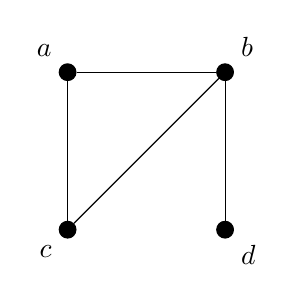
\begin{tikzpicture}

  % Small circles
  \node[draw, fill=black, circle, inner sep=0.075cm, label=above left:{$a$}] (circlea) at (0, 0) {};
  \node[draw, fill=black, circle, inner sep=0.075cm, label=above right:{$b$}] (circleb) at (2, 0) {};
  \node[draw, fill=black, circle, inner sep=0.075cm, label=below left:{$c$}] (circlec) at (0, -2) {};
  \node[draw, fill=black, circle, inner sep=0.075cm, label=below right:{$d$}] (circled) at (2, -2) {};

  % Arrows
  \draw[-] (circlea) to (circleb);
  \draw[-] (circlea) to (circlec);
  \draw[-] (circleb) to (circled);
  \draw[-] (circleb) to (circlec);

\end{tikzpicture}
\caption{\label{fig:Graph-Example}An Example of Graph}
\end{figure}

When a vertex $v$ serves as an endpoint of an edge $e$, it is said that $e$ is \emph{incident}\index{Incident edge} upon $v$. The \emph{degree}\index{Degree of a vertex} of a vertex $v$, notated as $\deg(v)$, corresponds to the count of edges incident on $v$. A vertex with degree zero is labeled as \emph{isolated}\index{Isolated vertex}, while a vertex with degree one is termed \emph{pendant}\index{Pendant vertex}. The \emph{neighborhood}\index{Neighborhood of a vertex} of a vertex $v$, signified by $N(v)$, includes all vertices that are adjacent to $v$. If $A \subset V$, the neighborhood of $A$ is given by $N(A) = \cup_{v \in A} N(v)$. A \emph{path}\index{Path} in a graph consists of a series of unique vertices $\{v_{0}, v_{1}, \ldots ,v_{k}\}$ such that $v_{i}$ and $v_{i+1}$ are adjacent for each $1 \leq i < k$. A path is known as a \emph{simple path}\index{Simple path} if no vertex is repeated. A graph is considered \emph{connected}\index{Connected graph} when a path exists between any two vertices. If $v_{0} = v_{k}$, the path is defined as a \emph{cycle}\index{Cycle}. A cycle is called a \emph{simple cycle}\index{Simple cycle} if it consists of at least three vertices and only the first and last vertices are repeated. 

\begin{example}
In a given graph $G=(V,E)$, the \emph{handshaking theorem}\index{Handshaking theorem} posits that $\sum_{v \in V} \deg(v) = 2m$, where $m = d(E)$, given that each edge has two endpoints.
\end{example}

If the vertex pairs $u, v$ are arranged in ordered pairs, the graph is termed a \emph{directed graph}\index{Directed graph}. In this case, $u$ is referred to as the \emph{initial vertex}\index{Initial vertex}, while $v$ is known as the \emph{terminal vertex}\index{Terminal vertex}. Given that $G$ is a directed graph, the \emph{in-degree}\index{In-degree of a vertex} of a vertex $v$, signified by $indeg(v)$, corresponds to the count of edges in which $v$ serves as a terminal vertex. The \emph{out-degree}\index{Out-degree of a vertex}, denoted by $outdeg(v)$, refers to the number of edges where $v$ is the initial vertex. A directed graph is \emph{strongly connected}\index{Strongly connected graph} if a directed path connects each pair of vertices. Directed graphs are typically illustrated with arrows, rather than lines, to represent edges.

A graph $G$ is classified as \emph{bipartite}\index{Bipartite graph} if the vertex set $V$ can be partitioned into two subsets $V_1$ and $V_2$ such that every edge of $G$ links a vertex from $V_1$ to one from $V_2$. Bipartite graphs are usually denoted as $G=(V_1, V_2, E)$. The degree of vertices in a bipartite graph adheres to the \emph{degree sum formula}\index{Degree sum formula}, $\sum_{u \in V_1} \deg(u) = \sum_{v \in V_2} \deg(v) = d(E)$.

A graph $G(V',E')$ is a \emph{subgraph}\index{Subgraph} of $G(V,E)$ if $V'$ is a subset of $V$ and $E'$ is a subset of $E$ with endpoints that belong to $V'$. A graph $G$ is termed a \emph{labeled graph}\index{Labeled graph} if its edges and/or vertices are assigned specific data. Specifically, if each edge $e$ of $G$ is allocated a nonnegative number $w(e)$, then $w(e)$ is referred to as the \emph{weight}\index{Weight of an edge} of $e$.

A specific type of graph that plays a fundamental role in this book is the \emph{tree}\index{Tree}. Defined as a non-empty graph, a tree ensures any pair of vertices are interconnected by a singular, unique path. A tree always includes a specially designated vertex termed the \emph{root}\index{Root of a tree}, and every edge of the tree is oriented away from the root.

\begin{example}
An alternative definition of trees, based on set theory, posits that a tree is a partially ordered set $(T, <)$ such that for each $t \in T$, the set $S = \{ s \in T : s < t \}$ possesses a least element – an element smaller than all other elements in $S$.
\end{example}

Given a tree $T$, for any vertex $v$ other than the root, the \emph{parent}\index{Parent of a vertex} of $v$ is the single, unique vertex $u$ such that an edge directly links $u$ to $v$. Conversely, if $u$ is the parent of $v$, $v$ is then identified as a \emph{child}\index{Child of a vertex} of $u$. Any other vertex within the tree sharing the same parent as $v$ is considered a \emph{sibling}\index{Sibling to a vertex} of $v$. The \emph{ancestors}\index{Ancestors of a vertex} of a vertex encompass all vertices along the path from the root to the given vertex, excluding the vertex itself but including the root. The \emph{descendants}\index{Descendant of a vertex} of a vertex $v$ include those vertices that count $v$ as an ancestor. A vertex with no children is labeled as a \emph{leaf}\index{Leaf vertex}, whereas vertices possessing children are referred to as \emph{branches}\index{Branches of a tree}. The \emph{depth}\index{Depth of a vertex} of a vertex $v$ is determined by the length of the unique path leading from the root to $v$. The \emph{height}\index{Height of a tree} of a tree is the maximum among the depths of all its vertices.

\begin{example}
For the tree illustrated in Figure \ref{fig:BinaryTree-Example}, the root vertex is $a$; $c$ serves as a parent of $d$, making $d$ a child of $c$; $d$ and $g$ are siblings; the ancestors of $d$ include $a$ and $c$; the descendants of $c$ comprise $d$, $e$, and $f$; leaf nodes in the tree are $b$, $e$, $f$, and $g$; $a$ and $c$ are branches; the depth of $d$ is 3; the height of the tree is 4.
\end{example}

\begin{figure}[t]
\centering
\begin{tikzpicture}

  % Small circles
  \node[draw, circle, inner sep=0.2cm, label=center:{$a$}] (circlea) at (0, 0) {};
  \node[draw, circle, inner sep=0.2cm, label=center:{$b$}] (circleb) at (-2, -2) {};
  \node[draw, circle, inner sep=0.2cm, label=center:{$c$}] (circlec) at (2, -2) {};
  \node[draw, circle, inner sep=0.2cm, label=center:{$d$}] (circled) at (0, -4) {};
  \node[draw, circle, inner sep=0.2cm, label=center:{$g$}] (circleg) at (4, -4) {};
  \node[draw, circle, inner sep=0.2cm, label=center:{$e$}] (circlee) at (-2, -6) {};
  \node[draw, circle, inner sep=0.2cm, label=center:{$f$}] (circlef) at (2, -6) {};


  % Arrows
  \draw[-] (circlea) to (circleb);
  \draw[-] (circlea) to (circlec);
  \draw[-] (circlec) to (circled);
  \draw[-] (circlec) to (circleg);
  \draw[-] (circled) to (circlee);
  \draw[-] (circled) to (circlef);

\end{tikzpicture}
\caption{\label{fig:BinaryTree-Example}An Example of a Tree}
\end{figure}

Given a vertex $v$ in a tree, the \emph{subtree}\index{Subtree} with $v$ as its root is the subgraph within the tree that includes $v$, its descendants, and all edges connected to these descendants. A tree is termed a \emph{k-ary tree}\index{k-ary tree} if each branch houses no more than $k$ children. If every branch comprises exactly $k$ children, the tree is then labeled a \emph{full k-ary tree}\index{full k-ary tree}. A \emph{k-ary} tree where $k=2$ is specifically referred to as a \emph{binary tree}\index{Binary tree}. A $k$-ary tree of height $h$ is deemed \emph{balanced}\index{Balanced tree} if all its leaves are located at a depth of $h$ or $h-1$.

\begin{example}
A tree composed of $n$ vertices includes $n-1$ edges. A full $k$-ary tree featuring $i$ branches hosts $m=ki+1$ vertices.
\end{example}

The procedure of visiting each node in a tree exactly once is defined as \emph{tree traversal}\index{Tree traversal}. The classifications of tree traversals are determined by the order of node visits, namely, \emph{depth-first} and \emph{breadth-first} order. In a depth-first traversal\index{Depth-first tree traversal}, the algorithm initiates at the root node and ventures as far as possible along each branch before transitioning to the next sibling. There are three standard strategies for processing nodes within the tree: \emph{in-order}\index{In-order tree traversal}, \emph{pre-order}\index{Pre-order tree traversal}, and \emph{post-order}\index{Post-order tree traversal}.

The following snippet of code, resembling C language syntax, demonstrates the usage of a recursive pre-order depth-first traversal algorithm to print a binary tree:

\begin{verbatim}
    void print_tree(binary_tree *tree) {
        if (!is_empty(tree)) {
            printf("%c\n",tree->node); /* print node */
            print_tree(tree->left_branch); /* process left branch */
            print_tree(tree->right_branch); /* process right branch */
        }
    }
\end{verbatim}

Conversely, in a breadth-first traversal\index{Breadth-first tree traversal}, the algorithm commences at the tree root and explores all nodes at the current depth before progressing to nodes at the subsequent depth level. Implementing depth-first tree traversal algorithms necessitates the employment of sophisticated data structures. For an example of such algorithms, please consult the references section.

\begin{example}
In the case of the tree delineated in Example \ref{ex:binary_tree}, a pre-order depth-first traversal would yield the string "abcdefg". Conversely, a pre-order breadth-first traversal would generate the string "abcdgef".
\end{example}

%
% Section: References
%

\section*{References}

The book "Discrete Mathematics" by Johnsonbaugh \cite{johnsonbaugh2009discrete} is tailored for undergraduate students taking a one- or two-semester course in discrete mathematics, thoroughly covering key topics in the field. "Introduction to the Theory of Computation" by Sipser \cite{sipser2012introduction} offers a comprehensive, clear, and student-centric introduction to the latest computational theory topics and methodologies. It is highly acclaimed for its in-depth exploration of automata, formal languages, and complexity theory. "Introduction to Algorithms" by Cormen et al. \cite{cormen1990introduction}, commonly known by the acronym "CLRS" derived from the authors' initials, is a seminal work in the algorithms field, encompassing a broad spectrum of topics, including graph algorithms. This book is both extensive and rigorous. Finally, "Matrix Computations" by Golub and Van Loan \cite{golub2013matrix} delves into various topics related to matrices, with an emphasis on matrix computations - an area of particular interest to those engaged in computational studies.






